% !TEX TS-program = pdflatex
% !TEX encoding = UTF-8 Unicode

\documentclass[preprint]{sigplanconf}

\usepackage{graphicx,listings,fixltx2e,lambda,array,multirow,color}


\begin{document}
\conferenceinfo{PLDI 2011}{June 4--8, 2011, San Jose, CA, USA.}
\copyrightyear{2010}

\preprintfooter{PLDI 2011}
\titlebanner{DRAFT---Do not distribute}

\title{Parakeet: General Purpose GPU Programming with Array Languages} 
% EDIT: old title was a bit wordy, looked gross, and "high level" is redundant if someone even glances at our abstract. 
%  --- General Purpose GPU Programming with High Level ArrayLanguages}

\authorinfo{Anonymous}{Anonymous}{Anonymous}
\lstset{ 
basicstyle=\small\footnotesize\ttfamily, % Standardschrift
numbers=left,                   % where to put the line-numbers
stepnumber=1,                   % the step between two line-numbers. If it's 1 each line 
numbersep=12pt,                  % how far the line-numbers are from the code
showspaces=false,               % show spaces adding particular underscores
showstringspaces=false,         % underline spaces within strings
showtabs=false,                 % show tabs within strings adding particular underscores
tabsize=2,	                % sets default tabsize to 2 spaces
captionpos=b,                   % sets the caption-position to bottom
breaklines=true,                % sets automatic line breaking
breakatwhitespace=false,        % sets if automatic breaks should only happen at whitespace
keywordstyle=\color{black}\bf,
%morekeywords={til,sum,sqrt,all, min, each, where, while,+,*,-,avg},            % if you want to add more keywords to the set
moredelim=[is][\itshape]{/*}{*/},
linewidth={\textwidth},
xleftmargin=20pt,
%framexleftmargin=17pt,
%framexrightmargin=5pt,
%framexbottommargin=4pt,
}

% define some useful commands to use in language specification 
\newcommand{\WITH}{\impfnt{with}}
\newcommand{\VALUES}{\impfnt{values}}
\newcommand{\MAP}{\impfnt{map}}
\newcommand{\REDUCE}{\impfnt{reduce}}
\newcommand{\ALLPAIRS}{\impfnt{allpairs}}
\newcommand{\CAST}{\impfnt{cast}}
\newcommand{\APPLY}{\impfnt{apply}}
\newcommand{\INDEX}{\impfnt{index}}
\newcommand{\SCAN}{\impfnt{scan}}
\newcommand{\THREADIDX}{\impfnt{threadIdx}}
\newcommand{\BLOCKIDX}{\impfnt{blockIdx}}
\newcommand{\BLOCKDIM}{\impfnt{blockDim}}
\newcommand{\GRIDDIM}{\impfnt{gridDim}}
\newcommand{\VEC}{\impfnt{vec}}
\newcommand{\concat}{\ensuremath{+\!\!\!\!+\,}}

\setlength\fboxsep{8pt}
\setlength\fboxrule{0.5pt}

\maketitle

\begin{abstract}
Contemporary GPUs offer staggering performance potential, which has
led to an explosion in recent work on enabling the execution of
general-purpose programs on GPUs. Despite various advances in making
general-purpose GPU programming easier, the two commonly used
frameworks (NVIDIA's CUDA and OpenCL) are cumbersome and require
detailed architectural knowledge on the part of the programmer to
fully harness this performance potential.

The potential performance advantage over contemporary CPUs that GPUs
offer is due in large part to their having been heavily optimized for
data parallel workloads.  Array-oriented programming--which encourages
the use of data parallel array operators (e.g.\ map, reduce, and
scan), and de-emphasizes the importance of explicit loops--is thus a
natural model for high level programming of GPUs.

We present Parakeet, an intelligent runtime for executing high level
array-oriented programs on GPUs.  The heart of Parakeet is an
interpreter, which upon reaching an array operator synthesizes and
executes a GPU program to implement that operator. Parakeet takes
advantage of runtime information both to choose between different
possible implementations of a GPU program and to set execution
parameters which greatly impact performance. Data is moved transparently
to and from the GPU, and garbage collected when no longer needed. 

We evaluate our system on two standard benchmarks: Black-Scholes
option pricing, and K-Means clustering.  We compare high level
array-oriented implementations to hand-written tuned GPU versions from
the CUDA SDK and the Rodinia GPU benchmark suite. Despite having
orders of magnitude less code, the high level
versions perform competitively when executed by Parakeet.
\end{abstract}

\section{Introduction}

Contemporary GPUs boast massive performance potential--in some cases orders of
magnitude higher performance per dollar than that of CPUs--and most desktop
systems today come with graphics processors.  This has led to an explosion in
recent work on enabling the execution of general-purpose programs on GPUs
(GPGPU) in order to harness this performance for non-graphics tasks
\cite{Cata10,Main10,Muns10,NvidCU,Sven08,Tard06}. Despite this, the two widely
used GPGPU frameworks--NVIDIA's CUDA \cite{NvidCU} and OpenCL
\cite{Muns10}--require the programmer to use extensive knowledge of low level
architectural details in order to fully harness the performance potential.

% Enable programmers to write GPGPU programs in productivity language
Our goal is to lower the barrier to GPGPU programming by allowing programmers to 
write in high level array languages are transparently compiled into efficient GPU programs. 
By ``array language'' we mean any language equipped with:
\begin{enumerate}
\item First-class array values
\item Succinct syntax for array creation/transformation
\item Idiomatic preference for bulk array operations instead of explicit loops
(``collection-oriented''~\cite{Sip91} programming)
\end{enumerate}

% Existing Array languages 
The prototypical array language is APL~\cite{Iverson62}, which allows for
extremely terse loop-free specification of algorithms. More commonly used array 
languages include Matlab~\cite{Moler80} (the lingua franca of signal processing
and machine learning research) as well as Python's NumPy~\cite{Oliphant07}
extensions. 


% Heart of Parakeet - an interpreter for our high level IL w/ array ops
In this paper, we present Parakeet, an intelligent runtime for executing high
level array programs on GPUs. Parakeet dynamically specializes user functions 
into a typed intermediate language and transparently executes array operations
on the GPU by synthesizing launching GPU kernels.


% Q front-end, agnosticism
We have implemented our first Parakeet front end for Q \cite{Borr08}, a
descendant of APL that is widely used in financial computing. 
Q is a nearly ``pure'' array language--its idiomatic style makes sparser use of
loops than even Matlab or NumPy--and is thus a natural first choice.
We are also currently working on front ends for both Matlab and Python.

% Performance
We evaluate Parakeet on two standard benchmark programs: Black-Scholes option
pricing and K-Means clustering.  We compare Q implementations of these
benchmarks run by Parakeet to hand-written, tuned GPU and CPU implementations
from the Rodinia \cite{Che09} and Parsec \cite{Bien08} benchmark suites and the
NVIDIA CUDA SDK \cite{NvidSD}.  Despite the Q implementations requiring orders
of magnitude fewer lines of code, our system delivers competitive performance.

% Bullet-point, drive-home contributions
The main contributions of this paper are the following:

\begin{itemize}
\item A working system in which programmers can write complex, high level code
that is automatically parallelized into efficient GPU programs.
\item A dynamic specialization algorithm that translates a significant subset of higher-order programs into efficient (unboxed, function-free) GPU code. 
\item A low-level intermediate language called \textit{Imp} which captures the notion of shapely computation \cite{Jay97} necessary in the absence of dynamic memory allocation.  
\item Evidence that dynamically compiling GPU programs can significantly
improve performance by taking advantage of runtime information to
tailor code and execution to runtime information.
\end{itemize}

\begin{figure*}[t!bh]
\begin{center}
\leavevmode
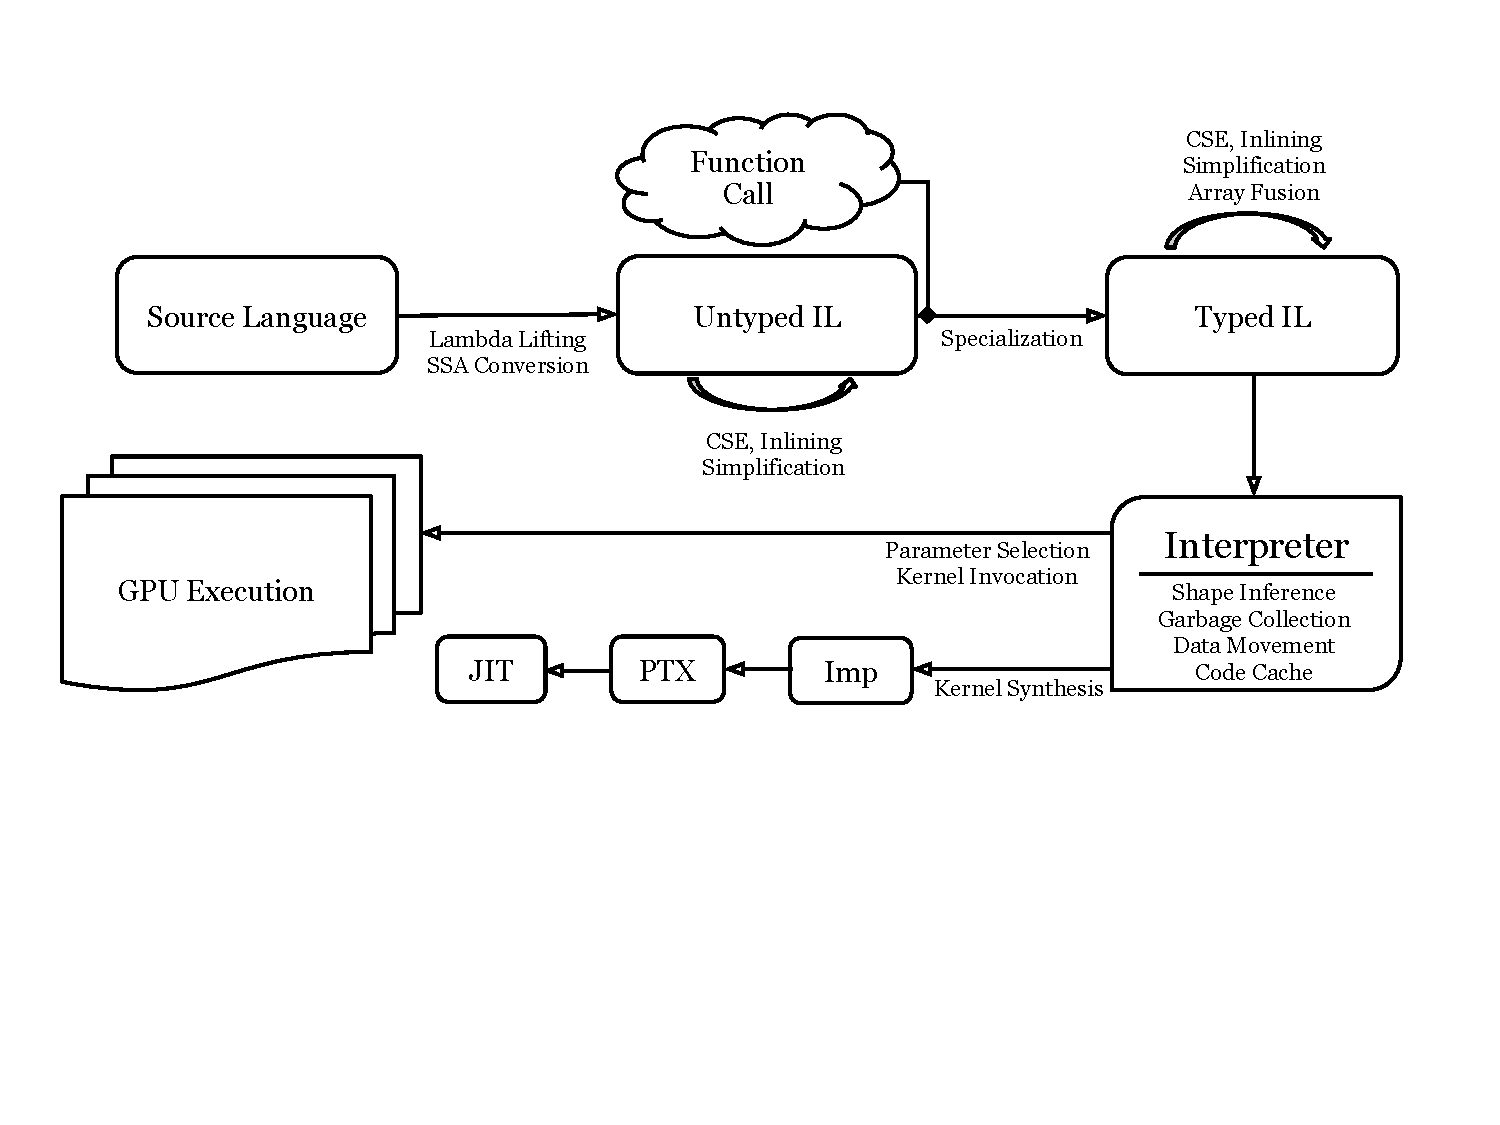
\includegraphics[scale=0.6, trim=10pt 180pt 10pt 120pt]{Pipeline.pdf}
\end{center}
\caption{Overview of Parakeet}
\label{fig:overview}
\end{figure*}
\section{Overview}


%Overview 
The pipeline of the execution of a program begins by the Parakeet system
intercepting function calls from the source language's interpreter and type
specializing them according to their argument types.  Parakeet then performs
various standard compiler optimizations on this IL form of the functions, as
well as fusion of array operators which is very beneficial for performance.
Parakeet then interprets the typed function, selectively executing array
operators either on the GPU or CPU. Parakeet synthesizes GPU
programs from a library of efficient array operator implementation skeletons,
with splice points where user-defined functions are inlined. Parakeet supports
the nesting of array operators, using heuristics to decide which level of
nesting should be compiled to GPU kernels, with the outer levels of nesting are
translated into iterative kernel invocations by our CPU runtime.  Data movement
and GPU garbage collection are handled transparently by Parakeet.



\section{Q: A High Level Array Language}
\label{Q}

While we emphasize that the Parakeet framework is built to be agnostic to source
array language, we chose to implement its first front end for Q, a high-level,
sequential array programming language from the APL family \cite{Borr08}.
Q is dynamically typed, and the standard proprietary implementation is
interpreted. Q is a natural choice for Parakeet, since idiomatic Q code uses
native array types and a rich set of array operators and higher-order
data parallel function modifiers that map well onto the Parakeet array
operators. Q is also a fully-featured language, with a large library of built-in
functions, and has a large user base in financial computing. Since our
focus is the Parakeet runtime, we omit many details of the Q language and only
present the salient features so as to illustrate the level of programming
and Q's support for array operators.

\subsection{K-Means Clustering Example}
\begin{figure}[h!]
\begin{lstlisting}
calc_centroid:{[X;a;i] avg X[where a = i]}
calc_centroids:{[X;a;k] 
  calc_centroid[X;a] each til k}
  
dist:{[x;y] sqrt sum (x-y) * (x-y)}
minidx:{[x] x ? min x}

kmeans:{[X;k;a]
  C: calc_centroids[X;a;k];
  converged: 0b;
  while[not converged;
    lastAssignment: a;
    D: X dist/:\: C;
    a: minidx each D;
    C: calc_centroids[X;a;k];
    converged: all lastAssignment = a];
  C}
\end{lstlisting}
\caption{K-Means Clustering implemented in Q}
\label{QKMeans}
\end{figure}

Let us illustrate Q with a full example: an implementation of K-Means
clustering.  K-Means is an algorithm for grouping data into some number of
clusters of nearby points in the multi-dimensional space formed by the
data's features.  These clusters are meant to help the user group the data
in a useful or meaningful way.  The
algorithm typically begins with a random initial assignment of the data points
to $k$ clusters. Then the algorithm proceeds iteratively, in each step first
calculating the center point (centroid) of each of the current clusters of data
points.  It then calculates the distances of all data points to each of these
new centroids and reassigns each point to its nearest cluster.  The algorithm
terminates either when the iteration doesn't change the assignments beyond some
given threshold, or when some fixed number of iterations has been reached.

In Figure \ref{QKMeans}, we see an implementation of K-Means in Q.  Five
functions are defined using Q's bracket notation for surrounding function
bodies and colon operator for assignment.  For example, the
\texttt{calc\_centroid} function on line 1 takes three parameters
\texttt{X}, \texttt{a}, and \texttt{i} (used as the input data matrix, the
current assignment vector, and the scalar index of the centroid to calculate,
respectively), and calculates that cluster's centroid.

In this function, we illustrate various aspects of the array-oriented nature of
Q. First, Q allows implicit mappings of functions elementwise across
vectors--for example, to test elementwise equality between the assignment
vector and the index \texttt{i}, we simply write \texttt{a = i}.  In addition,
this showcases Q's support for \emph{scalar promotion}.  In the statement
\texttt{a = i}, \texttt{a} is a vector of integers while \texttt{i} is a scalar
integer.  Semantically, Q implicitly promotes \texttt{i} to be a vector of the
value of \texttt{i} repeated a number of times equal to the length of \texttt{a}
and performs the elementwise equality between these two vectors.

We then generate the list of indices we want by applying the built-in
\texttt{where} operator to the result of this test, and index into the data
matrix \texttt{X} to get the list of data points in the centroid. The result of
this indexing is itself a 2-D matrix which contains the list of data points
belonging to the \texttt{i}-th cluster. Finally, the built-in \texttt{avg}
function--a reduction operator--gets applied to this 2-D list. Thus we see that
reductions and other built-in array operators can be applied to arrays of any
arity.  Further array built-ins used in K-Means include \texttt{sum},
\texttt{min}, and the find operator (denoted by `\texttt{?}').

In this algorithm we also see a number of higher-order data-parallel function
modifier keywords, which Q calls \emph{adverbs}.  For example, the \texttt{each}
keyword modifies a function by applying it elementwise to its argument.  In the
\texttt{calc\_centroids} function, we calculate each cluster's new centroid
by using \texttt{each} to apply the \texttt{calc\_centroid} function to a
list of integers from \texttt{0} to \texttt{k-1}.  The other adverb used in
K-Means is what we call \emph{all-pairs}, written `\texttt{/:\char`\\:}'.
(Technically all-pairs is a combination of two adverbs in Q--each-left and
each-right.) All-pairs modifies a binary function and applies it to each
pairs of elements from two input arrays.  We use all-pairs to apply the
\texttt{dist} function to each pair of data point and centroid to calculate all
the needed distances for reassigning the centroids.

As one can see, one is able to write compact and high level programs in Q
that manipulate arrays.  The CUDA implementation of K-Means in the Rodinia
benchmark suite is hundreds of lines of code long--our Q version is only 17,
and it could have been written even more compactly.

It is maybe worth pointing out that Q's representation of arrays is as vectors
of vectors, not as native multi-dimensional arrays?

\section{GPU Hardware Restrictions}
\begin{enumerate}
\item All values must be boxed (citation?)
\item No function pointers (is that true?)
\end{enumerate}

\section{Typed Intermediate Language}
In order to achieve good performance on a GPU it is necessary to ultimately eliminate indirection in the generated code. Simultaneously, there can be tremendous performance benefits to performing high level optimizations using the algebraic properties of array operators. Thus, our intermediate language must serve as a compromise between competing tensions: it must be sufficiently concrete to simplify later translation into function-free code but also abstract enough to facilitate fusion optimizations.  \\

The portion of a user's program which Parakeet executes is represented internally as flat sequence of non-recursive function definitions. 
We take inspiration from \cite{Bol09} and allow functions to both accept and return multiple values. This feature both supports optimization (by simplifying the specification of arity-raising and fusion transformations) and naturally models the simultaneous creation of multiple values on the GPU. By convention we will write $\overline{\tau_m}$ to denote a sequence of $m$ simple types, $\overline{v_n}$ for a sequence  of $n$ values, etc.. A single element is equivalent to a sequence of length 1 and sequences may be concatenated via juxtaposition, such that $\tau, \overline{\tau_n} = \overline{\tau_{m+1}}$. 

We draw attention to the types of closures, which are explicitly annotated with the types of their closed-over arguments. If one wished to arrive at this 
\begin{itemize}
\item It is worth noting that the programmer is limited to defining values with first-order types (data or functions which neither accept nor return function values). It is, however, possible to make use of primitive second-order operators such as $\mathbf{map}$ and $\mathbf{reduce}$. 
\item The accepted typing of closures involves existential types [find citation for typed closure conversion?], which are commonly implemented via boxing. Since our desire is to compile down to a final program without boxed values we instead annotate closures with the types of their implicitly carried arguments. This information is later used to transform closure invocation into a direct function call. 
\end{itemize}
\begin{tabular}{m{0.1cm}m{1.5cm}m{0.1cm}m{0.2cm}p{4.8cm}}
 \multicolumn{5}{l}{\textbf{Intermediate Language Syntax}}  \\[4pt]
& program & $p$ &  $\bnfdef$   &  $d_1 \cdots d_n $ \\[4pt]
& definition & $d$ & $\bnfdef$ & $f_i(\overline{x_m} : \overline{\tau_m}) \rightarrow (\overline{y_n} : \overline{\tau_n}) =s^{\small{+}}$ \\[4pt]
& statement  & $s$ & $\bnfdef$ & $\overline{x_m} : \overline{\rho_m} = e $\\[2pt]
&            &     & $\sep$    & $\IF \;v\; \THEN \;s^*\; \ELSE \;s^*$ \\[2pt]
&            &     & $\sep$    & $\WHILE \;e\; \DO \;s^+\;  $ \\[4pt]
& expression & $e$ & $\bnfdef$ & $ v_{f}(v_1, \ldots, v_m)$ \\[2pt]
&            &     & $\sep$    & $\textrm{values} (\overline{v_m})$ \\[2pt]
&            &     & $\sep$    & $\textrm{cast} \; (v, \tau)$ \\[2pt] 
&            &     & $\sep$    & $\MAP_m (v_{f},\overline{v_m})$ \\[2pt]
&            &     & $\sep$    & $\REDUCE_m (v_{f}, v_{g}, v_{init}, \overline{v_m})$ \\[2pt]
&            &     & $\sep$    & $\SCAN_m (v_{f}, v_{g}, v_{init}, \overline{v_m})$ \\[4pt]
& value      & $v$ & $\bnfdef$ & numeric constant\\[2pt]
&            &     & $\sep$    &  $x$  \quad \small{(data variable)} \\[2pt]
&            &     & $\sep$    &  $f$  \quad \small{(function label)} \\[2pt]
&            &     & $\sep$    &  $\oplus$ \quad \small{(scalar operator)} \\[2pt]
&            &     & $\sep$    &  $a$ \quad \small{(simple array operator)} \\[4pt]
\end{tabular}
\begin{tabular}{m{0.005cm}m{1.8cm}m{0.05cm}m{0.2cm}p{4.8cm}}
\multicolumn{5}{l}{\textbf{Type System}} \\[4pt]
& data     & $\tau$    & $\bnfdef$ & $int \sep float \sep \mathbf{vec} \; \tau   $ \\[4pt]
& closures        & $\rho$  & $\bnfdef$ & $\overline{\tau_{c}} \Rightarrow \overline{\tau_m} \rightarrow \overline{\tau_n}$\\[2pt]
&                 &           & $\sep$    & $\tau$ \\[4pt]
& higher-order    & $\theta$  & $\bnfdef$ & $\overline{\rho_m} \rightarrow \overline{\rho_n} $ \\[4pt]
\end{tabular}
Scalar operators include the usual boolean operations, scalar and floating point arithmetic, whereas examples of simple array operators include indexing, replication, and inspecting an array's shape. 
\\TODO: 
\begin{itemize}
\item Gated SSA (reference to Program Dependence Web?), explain gates in one sentence. 
\item Mention that $\MAP$ and friends are actually a family of operators parameterized by arity. 
\item What to do with reduce? The stream idea is wonky and not included in the type system. 
\end{itemize} 


\section{Translation, Specialization, and Optimization}
\label{Compilation}
To help elucidate the various transformation performed by Parakeet, we will define a distance function in Q and use it as a running example. 
\begin{figure}[h!]

    \begin{lstlisting}[numbers=none]
    dist: {[x;y] sqrt sum (x-y) * (x-y)}
    \end{lstlisting}
    \caption{Distance Function in Q}
\end{figure}[h!]

\subsection{Lambda Lifting and SSA Conversion } 
The first step in the Parakeet pipeline is a syntax-directed translation from a language-specific AST into Parakeet's IL.\\
Since type information is not yet available to specialize user functions, they must be translated into an untyped form (by setting all type assignments to $\bot$). 
The translation into Parakeet's IL maintains a closure environment and a name environment so that simultaneous lambda lifting and SSA conversion can be performed. 
Since we would like to interpret our intermediate language we use a gated SSA form based on the GSA sub-language of the Program Dependence Web \cite{Ott90}. Classical SSA cannot be directly executed since the $\phi$-nodes lack deterministic semantics. Gated SSA overcomes this limitation by using "gates" which not only merge data flow but also associate predicates with each data flow branch. Aside from simplifying certain optimizations, these gates also enable us to execute our code without converting out of SSA. 


\begin{figure}[h!]
\fbox{
\begin{tabular}{ m{0.1cm} m{6.7cm} }
  \multicolumn{2}{l}{dist $($ x, y $) \rightarrow  ($ z $) =$} \\
  & t$_1 = \mathrm{x} - \mathrm{y} $        \\
  & t$_2 = \mathrm{x} - \mathrm{y} $        \\
  & t$_3  = \mathrm{t}_1 * \mathrm{t}_2 $   \\
  & t$_4  = $sum$(\mathrm{t}_2) $           \\
  & z $  = \; \mathrm{sqrt}(\mathrm{t}_4)$   \\
\end{tabular}
}
\caption{Untyped Distance Function in SSA form}
\end{figure}



 
\subsection{Untyped Optimizations}
Parakeet performs optimizations at two distinct stages of translation pipeline-- before and after type specialization. We subject the untyped representation to inlining, common subexpression elimination and simplification (which consists of simultaneous constant propagation and dead code elimination). It is preferable to eliminate as much code as possible at this early stage since an untyped function body serves as a template for a potentially large number of future specializations. The only optimizations we do not perform on the untyped representation are array fusion rewrites, since these rely on type annotations to ensure correctness. 

\subsection{Specialization}
The purpose of specialization is to eliminate polymorphism, to make manifest all implicit behavior (such as coercion and scalar promotion), and to assign simple unboxed types to all data used within a function body. These goals are all essential for the efficient execution of user code on the GPU. 
\begin{enumerate}
\item polyvariance -- specialize a function for each distinct call string
\item signature elt is Type of DynType (for data) or Closure of (FnId.t, sig elt list) (for functions). Specialization isn't just on types! It's also on function tags and the types of their associated closure arguments. This is equivalent to performing defunctionalization (Reynolds) and then specializing exhaustively on the constant values of closure records. One caveat: non-constant closure values are disallowed to avoid explosive interpreter bloat on the GPU. Full higher-order programming on the GPU is theoretically possible, but unlikely. 
\item We only allow data to cross the boundary between our system and the source language. 
\end{enumerate}
Let's assume the \textit{dist} function is called with arguments of type $vec float$. The specializer will then generate the following code: 
\begin{figure}[h!]
\fbox{
  \begin{tabular}{m{0.1cm} m{6.7cm}}
    \multicolumn{2}{l}{dist $($ x $ : vec \; float $, y : $ vec \; float $) $ \rightarrow  ($ z $ :  vec \; float ) =$}  \\
    & t$_1   = \MAP ( -_{\mathrm{float}}, \mathrm{x}, \mathrm{y})$   \\
    & t$_2   = \MAP (*_{\mathrm{float}}, \mathrm{x}, \mathrm{y})$    \\
    & t$_3 = \REDUCE (+_{\mathrm{float}}, 0, \mathrm{t}_2)$          \\
    & z $  = \; \mathrm{sqrt}(\mathrm{t}_3)$                         \\
  \end{tabular}
}
\caption{Distance Function After Specialization}
\end{figure}
The actual intermediate language associates type annotations with every binding which we elide here for clarity. Note that the polymorphism inherent in math operations between dynamically typed values has been removed through the use of statically typed math operators. 


\subsection{Array Operator Fusion}
In addition to standard compiler optimizations (such as constant folding, function inlining, and common sub-expression elimination), 
we employ fusion rules\cite{Jones01} to combine array operators. Fusion enables us to minimize kernel launches, boost the computational density of generated kernels, and
avoid the materialization of unnecessary array temporaries. 
We present the fusion rules used by Parakeet in a simplified form, such that array operators only consume and produce a single value. Our rewrite engine actually generalizes these rules to use functions of arbitrary input and output arities, but we elide the full specification for the sake of clarity. 
\\[5pt]
\begin{tabular}{|m{0.001cm} m{0.05cm} p{6.75cm} p{0.05cm} |}
  \hline 
  & &  & \\
  & \multicolumn{2}{l}{\large{Map Fusion} }  &  \\[2.5pt]
  & & $\MAP(g, \MAP(f, x)) \leadsto \MAP(g \circ f, x)$ & \\
  & & & \\
  & \multicolumn{2}{l}{\large{Reduce-Map Fusion} }  & \\[2.5pt]
  & & $\REDUCE(g_r, g_{i}, \MAP(f, x)) \leadsto \REDUCE(g_r \circ f, g_{i} \circ f, x)$ & \\
  & & & \\
  \hline
\end{tabular}\\[4pt]
These transformations are safe if the following conditions hold: 
\begin{enumerate}
\item all the functions involved are referentially transparent
\item every output of the predecessor function ($f$) is used by the successor ($g$)
\item the outputs of the predecessor are used \textit{only} by the successor 
\end{enumerate}
The last two conditions are severe since they restricit our optimizer from rewriting anything but linear chains of produced/consumed temporaries. A large body of previous work\cite{Ald01} has demonstrated  both the existence of richer fusion rules and cost-directed strategies for applying those rules in more general scenarios. Still, despite the simplicity of our approach, we have observed that many wasteful temporaries in idiomatic array code are removed using the above rules. 
\\[5pt]
\begin{figure}[h!]

\fbox{
  \begin{tabular}{m{0.1cm} m{6.7cm} }
    \multicolumn{2}{l}{$\mathrm{f}_1 ($ acc : $ float $,  x $ : float $, y : $ float $) $ \rightarrow  ($ z $ :  float ) =$} \\
    & t$_1 = x - y $            \\
    & t$_2  = t_1 * t_1 $       \\
    & z $ = $ acc $+$ t$_2$     \\
    &  \\ 
  \multicolumn{2}{l}{$\mathrm{dist} ($ x $ : vec \; float $, y : $ vec \; float $) $ \rightarrow  ($ z $ :  vec \; float ) =$} \\
  & t$_3 = \REDUCE (\mathrm{f}_1, 0.0, \mathrm{x}, \mathrm{y})$   \\
  & z $ = \mathrm{sqrt}(\mathrm{t}_3)$  \\
  \end{tabular}
}
\caption{Distance Function After Fusion Optimization}
\end{figure}



\section{GPU Code Generation}
\subsection{CUDA Programming Model}

In this section we give an overview of modern GPU architecture and the CUDA
programming model.  Modern graphics processors are made up of hierarchical
arrays of simple processors, with each level of the hierarchy sharing some
commmon hardware resources.  When performing graphics computations these
processors execute shader programs for performing rendering tasks.  With the
advent of GPGPU programming environments such as NVIDIA's CUDA \cite{NvidCU} and
OpenCL \cite{Muns10}, programmers can execute general-purpose programs directly
on these processors as well.

The current back end for Parakeet targets the CUDA platform by emitting PTX, the
pseudoassembly language in which CUDA programs are ultimately implemented.
In CUDA, a program is organized into {\it kernels} and {\it host} code.
Kernels are sequential code that is run by typically many thousands of ultra
lightweight threads on the GPU's, or {\it device}'s, processors.  Host code is
the code run on the CPU. Typically, a host thread launches a kernel onto the
GPU, waits for results, and then potentially launches further kernels.

A CUDA kernel's threads are organized into {\it thread blocks}, which are groups
of at most a few hundred threads that can communicate and share local resources.
Threads within a block can perform barrier synchronizations with each other via
a CUDA intrinsic, but threads from different blocks have no way to perform
synchronization other than for the kernel to terminate.  Thus algorithms that
require global synchronization must be broken up into multiple kernel launches,
each of which incurs a small fixed performance overhead.  The body of a
kernel can be written so as to be agnostic to the number of threads and
blocks with which it is launched, with the programmer specifying at runtime how
many thread blocks are required and how many threads to launch per block. This
allows the kernel programs to be scalable to different datasizes without
requiring them to be rewritten. The standard idiom is for each thread to be
assigned a small computation to be performed on a small subset of some large
input data set.  The threads are each assigned a unique index in the kernel's
{\it grid} of threads, which is used to determine the data for which they are
responsible.

The GPU consists of a series--typically a few hundred--simple processors that
are organized into small groups (on current chips between 8 and 48) of
processors called {\it symmetric multiprocessors} or SMs.  SMs form the basic
hardware scheduling unit, with processors within an SM sharing instruction
fetch and decode units and thread blocks executing in their entirety on a
single SM.

At the lowest level of the processor hierarchy are symmetric
processors or SPs, which are very simple sequential processors.  At the
next level are symmetric multiprocessors or SMs, which are groups of 8 SPs that
share an instruction issue and decode unit.  This means that all SPs within an
SM execute their instructions in lockstep.  In the CUDA model, thread blocks are
scheduled to run in their entirety on a single SM.  The SPs are then grouped to
share texture processing units, and then these groups along with L2 caches make
up the GPU chip.  The graphics card bundles the GPU along with a large block of
off-chip DRAM, typically on the order of a few gigabytes in modern cards.

The CUDA model is a Single Instruction Multiple Thread or SIMT model, meaning
that multiple threads with a block each execute the same instruction at the same
time.  This differs from SIMD models in that branching instructions are allowed
which diverge with a thread block.  However, this results in a significant
performance degradation, as all threads in the block are then forced to execute
both paths of the branch, with logical noops being executed by the threads on
the path which didn't satisfy their conditional test.

In order to get maximum performance on a GPU, it is very important to manage
memory usage.  While the peak memory bandwidth on modern GPUs is up to 150GB/sec
or more--up to an order of magnitude higher than that of CPUs--this bandwidth
can only be reached with careful access patterns on the part of threads within a
block.  In addition, each SM has a 16KB scratchpad called {\it shared memory}.
The programmer must explicitly manage shared memory, and careful usage of it can
result in orders of magnitude performance improvements over naively-written CUDA
programs.  Further, data must be manually moved between system RAM and the
graphics card's DRAM.  Modern GPUs use PCI-Express, which has a maximum transfer
rate of around 4GB/sec, which can easily become the major bottleneck in CUDA
programs if memory transfers aren't managed carefully.  Finally, graphics cards
tend to have limited global memory (typically between 500MB and 2GB), and a
user's windowing system can consume much of this on its own (on our office
desktops, X Windows tends to consume around 600MB).  Thus GPU RAM is an
important scarce resource to be managed.

Various constraints limit how a programmer can structure his or her CUDA
programs.  Each SM is able to execute a maximum of 8 thread blocks and
a maximum of 768-1536 threads at a time.  In addition, a group of thread blocks
can be co-scheduled on an SM only if they consume at most 8K-32K registers, as
each SM shares a register pool.  Finally, no more than 16-48KB of shared
memory per SM can be used at a time, and so thread blocks which in aggregate
exceed this limit cannot be co-scheduled.

The complexity of programming in the CUDA platform should be evident.  Parakeet
aims to manage these low level details efficiently and transparently for the
programmer.

%\subsection{GPU Memory Management}
%
%When
%Parakeet synthesizes a GPU program, it first determines whether the input and
%output arguments for that program will fit in their entirety in the available
%GPU memory.  Typically, GPUs have around 500MB to 2GB of RAM, and a significant
%portion of this can be taken up by a user's windowing system.  (In our
%experiments, on a card with 896MB of memory, X Windows can consume well over
%600MB on its own during simple office usage.)  If the data does fit, Parakeet
%copies whatever inputs are not already on the GPU to it and allocates storage
%for the output.  If not, Parakeet chunks the data up into manageable portions,
%copying down one section at a time to the GPU, and then transfering the
%partial result back to the CPU to build the complete result.


\subsection{Imp}
Important characteristics (ways Imp is more expressive than CUDA):
\begin{enumerate}
\item  Arrays are not associated with a particular GPU memory space (global, texture, constant, etc..), allowing us to compile variants of an Imp kernel where inputs reside in different memory spaces. 
\item Local temporaries can be arrays in addition to scalars. This generalizes CUDA's use of "local" memory for spilled scalar variables. 
\item Space requirements of a function call (all outputs and local arrays it must allocate) can be determined as a function of input sizes. This is necessary for GPU computations only have access to memory which is allocated before their launch and cannot "dynamically" allocate more memory. 
\end{enumerate}
\begin{tabular}{m{0.1cm}m{1.2cm}m{0.1cm}m{0.2cm}p{2cm}p{2.7cm}}
 \multicolumn{6}{l}{\textbf{Imp Language Syntax}} \\[4pt]
& definition        & $d$      & $\bnfdef$ & 
      \multicolumn{2}{l}{$f(\overline{x_m} : \overline{\tau_m}) \rightarrow (\overline{y_n} : \overline{\tau_n}, \overline{\sigma_n}) = s^{\small{+}}$} \\[4pt]
& shape             & $\sigma$ & $\bnfdef$ & $ [] $                                            &  \quad \small{(shape of scalar)}      \\[2pt]
&                   &          & $\sep$    & $ \sigma \concat \sigma $                         &  \quad \small{(concatenate)}      \\[2pt]
&                   &          & $\sep$    & $ [z] $                                           &  \quad \small{(singleton)}   \\[2pt]
&                   &          & $\sep$    & $ \sigma[\mathrm{const} \ldots  \mathrm{const}] $ &  \quad \small{(slice)}       \\[4pt]
& size              & $z$      & $\bnfdef$ & $ \mathrm{dimsize}(x_i, \mathrm{const}) $         &  \quad \small{(input dimension)}   \\[2pt]
&                   &          & $\sep$    & $ \mathrm{rank}(x_i) $                            &  \quad \small{(input rank)}  \\[2pt]
&                   &          & $\sep$    & $ \oplus(\overline{z_m})$                         &  \quad \small{(scalar primitive)}    \\[2pt]
\end{tabular}
\begin{tabular}{m{0.1cm}m{1.2cm}m{0.1cm}m{0.2cm}p{4.7cm}}
& statement         & $s$      & $\bnfdef$ & $x : \tau, \sigma = e $         \\[2pt]
&                   &          & $\sep$    & $\IF \;v\; \THEN \;s^*\; \ELSE \;s^*$ \\[2pt]
&                   &          & $\sep$    & $\WHILE \;e\; \DO \;s^+\;  $ \\[4pt]
& expression        & $e$      & $\bnfdef$ & $\oplus(\overline{v_m})$ \\[2pt]
&                   &          & $\sep$    & $v_{array}[\overline{v_m}]$ \\[2pt]
&                   &          & $\sep$    & $\textrm{cast} \; (v, \tau)$ \\[2pt] 
&                   &          & $\sep$    & $\textrm{dimsize}(v_{array}, v_{int}) $ \\[2pt]
&                   &          & $\sep$    & $v$ \\[4pt]
& value      & $v$ & $\bnfdef$ &  $x$ \\[2pt]
&            &     & $\sep$    &   numeric constant \\[2pt]
&            &     & $\sep$    &  $\mathrm{threadIdx.\{x|y|z\}} $\\[2pt]
&            &     & $\sep$    &  $\mathrm{blockIdx.\{x|y|z\}} $\\[2pt]
&            &     & $\sep$    &  $\mathrm{blockDim.\{x|y|z\}} $\\[2pt]
&            &     & $\sep$    &  $\mathrm{gridDim.\{x|y\}}    $\\[2pt]
\end{tabular}
Here is a simple example of an Imp kernel template: 

\section{Evaluation}
\label{Evaluation}

We evaluated Parakeet on two standard benchmark programs: Black-Scholes option
pricing, and K-Means Clustering.  We compare Parakeet against both hand-tuned
CPU and GPU implementations.  For Black-Scholes, the CPU implementation is
taken from the PARSEC \cite{Bien08} benchmark suite--which we used as the basis
of our Q implementation--and the GPU implementation is taken from the CUDA SDK
\cite{NvidSD}.  For K-Means Clustering, we wrote our own Q version in 17 lines
of code.  Both the CPU and GPU benchmark version come from the Rodinia
benchmark suite \cite{Che09}.

Our experimental setup is as follows.  We ran the CPU benchmarks on a machine
with 3 Intel Nehalem 2.67GHz X5650 4-core CPUs (for a total of 12 cores) with
24GB of RAM.  The peak throughput of this machine is thus 32GLOP/s, and it has
a peak memory bandwidth of 32GB/s.

For all GPU benchmarks, we ran the programs on both an NVIDIA GTX2XX and an
NVIDIA GTX460.  The GTX2XX has 240 processor cores with clock speeds of
Y.YY GHz and YMB of memory, with peak execution throughput of Y.YY GFLOP/s and
peak memory bandwidth of Y.YY GB/s.  The GTX460 has 336 processor cores with
clock speeds of 1.35GHz and 1GB of memory, and has a peak execution throughput
of 907 GFLOP/s and a peak memory bandwidth of 115.2 GB/s.

For our Parakeet benchmarks, the desktop system we used had a BLAH processor
with BLAH specs.

\subsection{Black-Scholes}
Black-Scholes option pricing \cite{Blac73} is a standard benchmark for data
parallel workloads, since it is embarrassingly parallel--the calculation of the
price of a given option doesn't impact that of any other, and the benchmark
consists of simply running thousands of independent threads in parallel for
computing the prices of thousands of options.

We compare our system against the multithreaded OpenMP CPU implementation
from the PARSEC \cite{Bien08} benchmark suite for 1 to 12 threads and 


\subsection{Dynamic Tuning}
In order to test the effects of our dynamic tuning optimizations, 

\section{Related Work}
\label{RelatedWork}

% ALEX: put the skeletons and vaguely related stuff first and then focus on Nikola, Accelerate and Copperhead? 
Our approach is very similar in spirit to that of the skeletal programming
community \cite{Cole04}.  We both seek to use generic parallel programming
constructs which capture most of the common parallel patterns in a concise and
easy-to-use language.  

%ALEX: I like the idea of a chronological presentation: Vertigo, Accelerator, Accelerator, Nikola, Copperhead
There has also been other work directed specifically at raising the level of
abstraction above that of CUDA and OpenCL for doing GPGPU programming.  Conal
Elliot's Vertigo \cite{Elli04} was a declarative parallel language embedded in
Haskell which was used for GPGPU programming.  It was designed for older GPUs
(pre-CUDA), and only parallelized map computations (not handling, for example,
parallel reductions or all-pairs type computations).  Microsoft's Accelerator
\cite{Tard06} is a declarative GPU language embedded in C\# which creates a
directed acyclic graph of LINQ operations--a collection of common data querying
operations such as filtering, grouping, and joining--and compiles them to
(pre-CUDA) shader programs.  

Our work is most closely related to Copperhead \cite{Cata10}, which also uses data parallel
operators to dynamically compile a high level language into GPU programs. Where we explicitly
specialize functions to uncover unboxed representations, Copperhead reuses the machinery 
of C++ templates for specialization. Furthermore, where we have created our own GPU kernel 
templates within the Imp DSL, Copperhead calls into the data parallel operators of the Thrust
library for C++. Extensive reliance on a C++ backend is a double-edged sword, invocation of
C++ template compilations can result in unfavorably long delays at runtime. Unlike Copperhead,
Parakeet does not require the programmer to specify their computation in a purely functional manner.
Our system allows for both looping and variable reassignment. The only restriction is that a function
must be both referentially transparent and shapely in order to run on the GPU when passed to an array
operator (otherwise in runs on the CPU). Furthermore, we do not expect the programmer to code directly
in our intermediate language, but rather perform an initial specialization phase which desugars
a more expressive untyped language (for example, turning array arithmetic into explicit maps). 
\section{Conclusion}
\label{Conclusion}

We have presented Parakeet, an intelligent runtime for executing high level
array-oriented programs on GPUs.  Parakeet alleviates programmers from having
to write code that explicitly manages low level architectural details, pushing
the level of abstraction for GPGPU programming up to the level of productivity
languages.  Parakeet automatically synthesizes GPU programs from data parallel
array operators, transparently running these programs and moving data back and
forth to the GPU's memory and performing GPU memory garbage collection.
Parakeet includes a series of optimizations to generate more efficient GPU
programs, including array operator fusion and the use of shared and texture
memory on the GPU.  Parakeet is a working system, in which complex programs can
be written and executed efficiently.  On two benchmark programs, Parakeet
delivers performance competitive with even hand-tuned CPU and GPU
implementations.

In future work, we hope to support more front ends and back ends.  At the
moment, we are building front ends for both Matlab and Python.  We envision
building a back end for multicore CPUs as well, likely targeting LLVM
\cite{Latt02}.

\bibliographystyle{acm}
\bibliography{../Parallelism}{}

\end{document}
